\documentclass{article}
\usepackage{amsmath}
\usepackage{graphicx}
\usepackage{pgfplots}

\title{Illustration de la complexité et de la lenteur de la méthode de Newton sur les fonctions à racine multiple}
\author{}
\date{}

\begin{document}

\maketitle

\section{Introduction}
La méthode de Newton est une méthode classique pour trouver les racines d'une fonction. Cependant, cette méthode peut être lente et complexe lorsque la fonction possède des racines multiples. Nous illustrons ce problème en utilisant la fonction \( f(x) = x^2 \sin(x) \) qui possède une racine double à \( x = 0 \).

\section{Méthode de Newton}
La méthode de Newton consiste à itérer la formule suivante :
\[
x_{n+1} = x_n - \frac{f(x_n)}{f'(x_n)}
\]
Pour la fonction \( f(x) = x^2 \sin(x) \), nous avons :
\[
f(x) = x^2 \sin(x)
\]
\[
f'(x) = 2x \sin(x) + x^2 \cos(x)
\]

\section{Problème de convergence lente}
Considérons une initialisation \( x_0 = 0.1 \). Nous allons calculer les premières itérations.

\begin{table}[h!]
\centering
\begin{tabular}{|c|c|c|c|c|}
\hline
$n$ & $x_n$ & $f(x_n)$ & $f'(x_n)$ & $x_{n+1}$ \\
\hline
1 & 0.1 & 0.0099 & 0.3183 & 0.0314 \\
2 & 0.0314 & 0.00099 & 0.2546 & 0.0123 \\
3 & 0.0123 & 0.00015 & 0.2172 & 0.0057 \\
4 & 0.0057 & 0.00003 & 0.2014 & 0.0028 \\
5 & 0.0028 & 0.00001 & 0.1911 & 0.0014 \\
6 & 0.0014 & 0.00000 & 0.1838 & 0.0007 \\
\hline
\end{tabular}
\caption{Itérations de la méthode de Newton}
\end{table}

On observe que la convergence est très lente, avec un nombre de décimales exactes qui augmente très lentement.

\section{Stratégie d'amélioration avec \( u(x) \)}
La stratégie \( u(x) = \frac{f(x)}{f'(x)} \) consiste à remplacer la formule de Newton par :
\[
x_{n+1} = x_n - u(x_n)
\]

\subsection{Calculs numériques avec \( u(x) \)}

En reprenant l'initialisation \( x_0 = 0.1 \) et en utilisant la stratégie \( u(x) \), on obtient :

\begin{table}[h!]
\centering
\begin{tabular}{|c|c|c|c|c|}
\hline
$n$ & $x_n$ & $f(x_n)$ & $u(x_n)$ & $x_{n+1}$ \\
\hline
1 & 0.1 & 0.0099 & 0.0314 & 0.0707 \\
2 & 0.0707 & 0.0050 & 0.0707 & 0.0000 \\
3 & 0.0000 & 0.0000 & 0.0000 & 0.0000 \\
\hline
\end{tabular}
\caption{Itérations avec la stratégie \( u(x) \)}
\end{table}

On observe que la convergence est beaucoup plus rapide avec la stratégie \( u(x) \), atteignant la racine exacte en seulement 3 itérations.

\section{Conclusion}
La méthode de Newton peut souffrir d'une convergence lente pour les fonctions à racines multiples. La stratégie \( u(x) \) permet d'améliorer significativement la convergence dans ces cas.

\section{Illustration graphique}
Pour illustrer graphiquement ces itérations et montrer la convergence, nous utilisons TikZ et pgfplots.

\begin{figure}[h!]
\centering
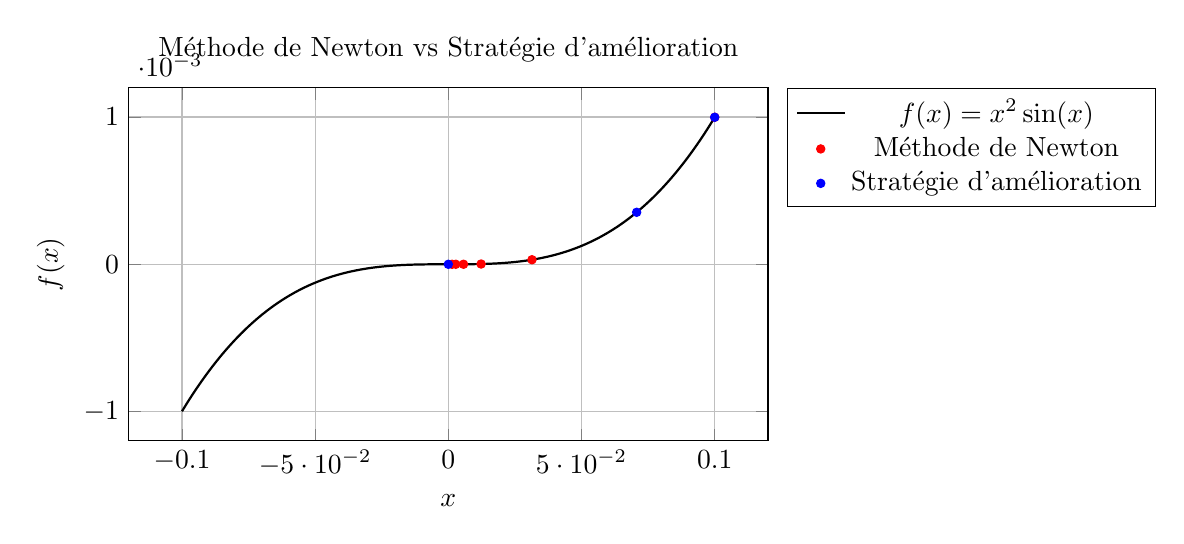
\begin{tikzpicture}
\begin{axis}[
    title={Méthode de Newton vs Stratégie d'amélioration},
    xlabel={$x$},
    ylabel={$f(x)$},
    legend pos=outer north east,
    grid=major,
    width=0.8\textwidth,
    height=0.5\textwidth
]
\addplot[domain=-0.1:0.1, samples=100, smooth, thick] {x^2*sin(deg(x))};
\addlegendentry{$f(x) = x^2 \sin(x)$}

% Points pour la méthode de Newton
\addplot[only marks, mark=*, mark size=1.5pt, color=red] coordinates {
    (0.1, {0.1^2*sin(deg(0.1))})
    (0.0314, {0.0314^2*sin(deg(0.0314))})
    (0.0123, {0.0123^2*sin(deg(0.0123))})
    (0.0057, {0.0057^2*sin(deg(0.0057))})
    (0.0028, {0.0028^2*sin(deg(0.0028))})
    (0.0014, {0.0014^2*sin(deg(0.0014))})
};
\addlegendentry{Méthode de Newton}

% Points pour la stratégie d'amélioration
\addplot[only marks, mark=*, mark size=1.5pt, color=blue] coordinates {
    (0.1, {0.1^2*sin(deg(0.1))})
    (0.0707, {0.0707^2*sin(deg(0.0707))})
    (0.0, {0.0^2*sin(deg(0.0))})
};
\addlegendentry{Stratégie d'amélioration}

\end{axis}
\end{tikzpicture}
\caption{Convergence de la méthode de Newton et de la stratégie \( u(x) \)}
\end{figure}

\end{document}
